\subsection{Séquenceurs}

\subsubsection{Présentation générale}

Les deux étages de la fusée SP-02 sont chacun équipés d’un séquenceur embarqué identique, développé pour gérer de manière
autonome l’ensemble des événements critiques du vol et assurer la conformité au \acrshort{CDC} Fusex. Cette architecture
commune facilite la fabrication, les essais et la maintenance, tout en permettant une configuration logicielle propre à chaque
étage.\\

\begin{figure}[h!]
    \centering
    \begin{subfigure}{0.45\textwidth}
        \centering
        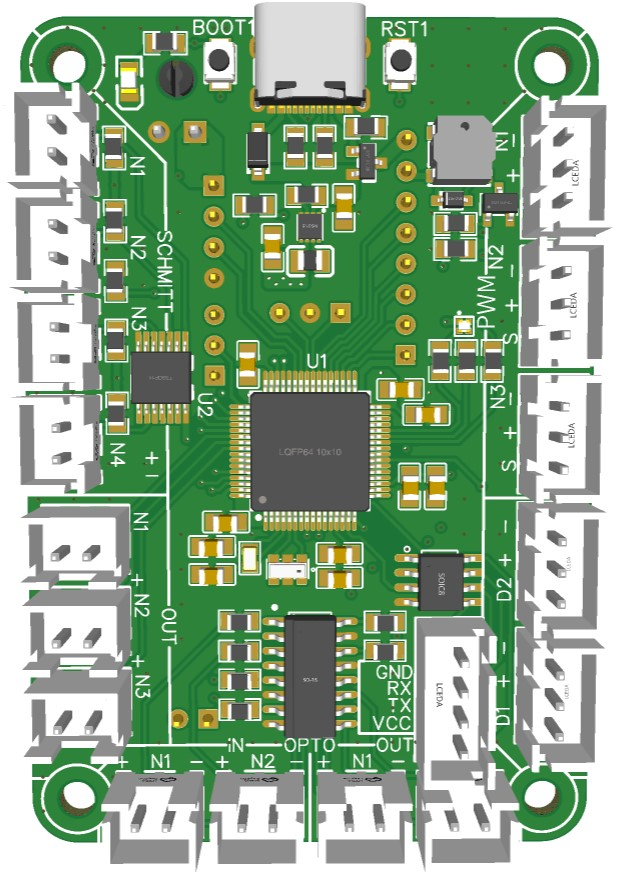
\includegraphics[width=0.75\textwidth]{figures/elec/PCB_Sequenceur_front.jpg}
        \caption{face avant}
        \label{fig:PCB_Sequenceur_front}
    \end{subfigure}
    \hfill
    \begin{subfigure}{0.45\textwidth}
        \centering
        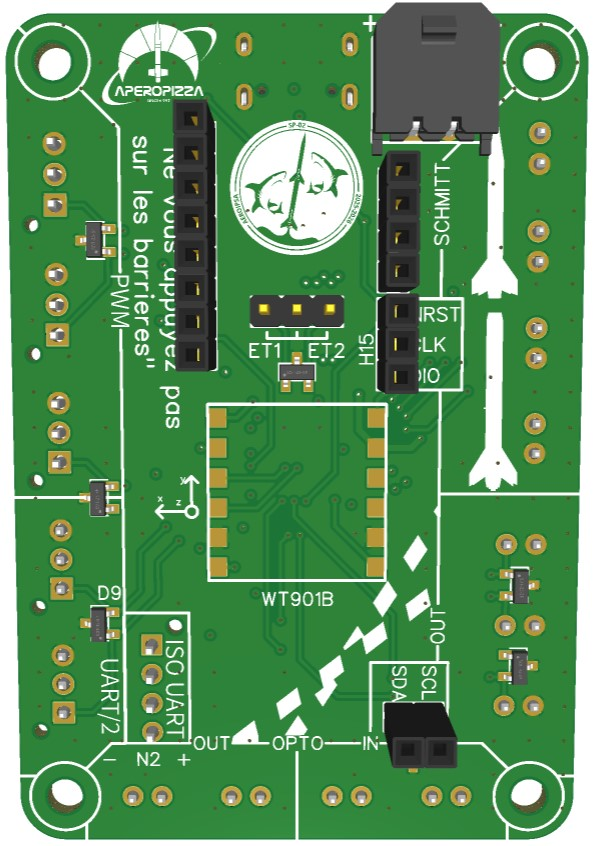
\includegraphics[width=0.75\textwidth]{figures/elec/PCB_Sequenceur_back.jpg}
        \caption{face arrière}
        \label{fig:PCB_Sequenceur_back}
    \end{subfigure}
    \caption{Rendu 3D de la carte séquenceur}
    \label{fig:PCB_Sequenceur}
\end{figure}

La face avant de la carte séquenceur (\ref{fig:PCB_Sequenceur_front}) est le côté dirigé vers l'intérieur de la fusée, tandis
que la face arrière (\ref{fig:PCB_Sequenceur_back}) est orientée vers l'extérieur. Ainsi l'ensemble des connecteurs, hormis ceux
de la batterie et de ceux de la carte \acrshort{IHF}, sont orientés vers l'intérieur de la fusée pour faciliter l'intégration.
Ceux de la carte \acrshort{IHF} sont orientés de telle sorte à ce que cette dernière soit accessible depuis l'extérieur de la fusée.

\vspace{0.2cm}

\hspace*{-\parindent}%
\begin{minipage}{0.60\textwidth}
    \noindent Chaque séquenceur assure notamment :
    \begin{itemize}
        \item la détection du décollage via la coupure de la boucle \textit{jack} ;
        \item le démarrage du chronomètre interne servant de référence aux fenêtres temporelles ;
        \item le pilotage du système de récupération (parachute, trappe) ;
        \item la supervision de la séparation inter-étage et l’inhibition des actions en cas d’anomalie. \\
    \end{itemize}

    Le séquenceurs du première étage devra en plus se charger :
    \begin{itemize}
        \item du pilotage du système d'aérofreins ;
        \item du déverrouillage du mécanisme de séparation. \\
    \end{itemize}

    Le séquenceur du second étage devra quant à lui gérer :
    \begin{itemize}
        \item de la détection de l'attitude de la fusée ;
        \item de l'allumage du moteur du second étage.
    \end{itemize}
\end{minipage}
\hfill
\begin{minipage}{0.4\textwidth}
    \begin{figure}[H]
        \centering
        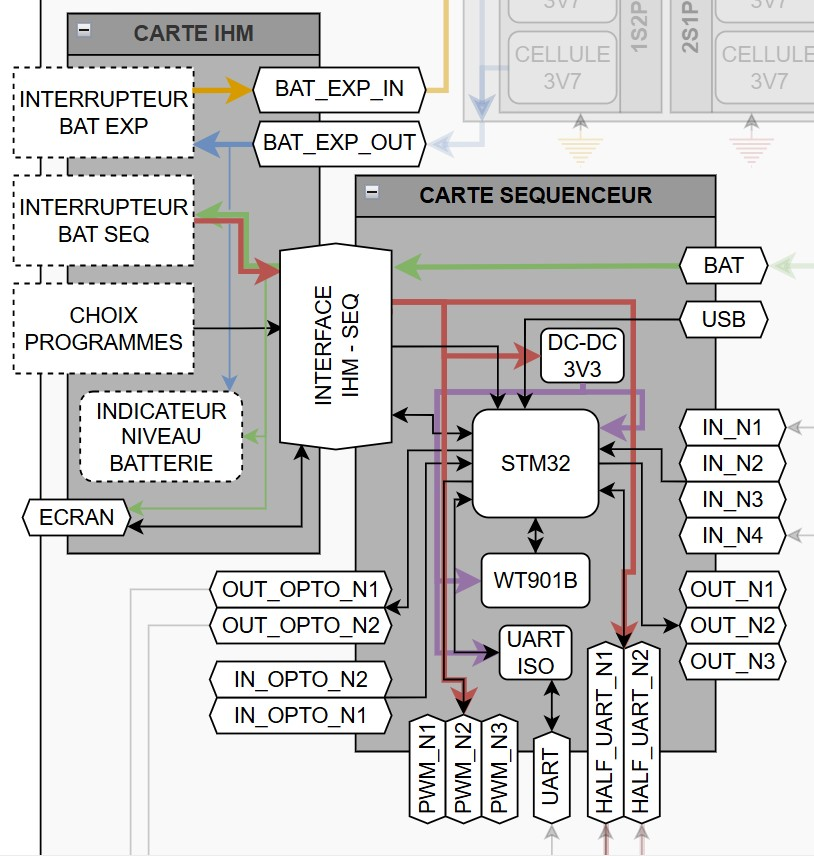
\includegraphics[width=\textwidth]{figures/elec/synopsis_sequ.jpg}
        \caption{Zoom sur le séquenceur et interface}
        \label{fig:synopsis_sequ}
    \end{figure}
\end{minipage}

\vspace{0.5cm}

Le synopsis figure \ref{fig:synopsis_sequ} présente le séquenceur ainsi que la carte interface.

\newpage

\subsubsection{Architecture matérielle}

\subsubsubsection{Entrées / sorties}

La carte intègre :
\begin{itemize}
    \item 1 connecteur Molex Micro-Fit 3.0 pour la batterie
    \item 4 entrées conditionnées par portes à hystérésis de type \textit{Schmitt trigger} précédé par des résistances
    pull-up. Elles sont utilisées pour la détection d’événements discrets tels que décollage et la séparation.  
    \item 3 sorties directement connectées à 3 \acrshort{GPIO} du microcontrôleur utilisées par exemple pour transmettre le
    signal d'allumage du 2e étage.
    \item 2 entrées logiques optocouplées destinées à des liaisons vers d'autres équipement de manière sécurisés ;
    \item 2 sorties logiques optocouplées destinées à des liaisons vers d'autres équipement de manière sécurisés ;
    \item 2 liaisons \acrshort{UART} dont une dédiée à la centrale inertielle \verb|WT901B| et un autre pour la liaison avec
    l'expérience et préalablement découplé via un module \verb|ADUM1281ARZ-RL7|;
    \item 2 liaison \acrshort{UART} half-duplex\footnote{La variante half-duplex de l'\acrshort{UART} désigne une configuration
    où les données TX et RX sont transmit dans un seul câble au lieu de 2 dans la version classique dite "full-duplex.} servant
    au pilotage des servomoteurs Feetech ;
    \item 3 liaison \acrshort{PWM} servant de connecteurs de secours au développement de l'architecture système global ;
    \item 4 connecteurs dupont verticaux femelle servant à la connexion de la carte \acrshort{IHF} ;
    \item 1 jumper de configuration pour la séléction du mode de fonctionnement du séquenceur (1er étage ou 2e étage) ;
    \item 1 port \acrshort{USB} type C pour l'alimentation de la carte sans batterie et pour le développement du programme
    logiciel embarqué.
\end{itemize}

A noter qu'un bon nombre des connecteurs ne sont pas utilisé nominalement sur le projet SP-02. Ils ont cependant été mis et
gardé au cours du développement afin de guarentir une agilité face à des problématiques qui pourront ou qui auraient pu
arrivé nécessitant des changements au niveau de l'architecture système global.  

\subsubsubsection{Alimentation électrique}
\label{subsubsubsec:sequenceur_alimentation}
Le séquenceur est alimenté par deux batteries Li-ion 18650 de 2600 mAh mis en série et fournissant une tension nominale de 7,4 V.
La puissance de la batterie passe par le connecteur Molex Micro-Fit 3.0, puis par la carte \acrshort{IHF} via les dupont
vecticaux et dans un interupteur mécanique. Ce dernier permet de contrôler l'alimentation du séquenceur depuis l'extérieur de la
fusée. L'alimentation retourne ensuite vers le séquenceur et passe par un régulateur de tension \verb|TPS6217| pour fournir une
tension de 3.3 V au microcontrôleur et aux autres composants de la carte. Le régulateur est capable de fournir un courant de
500 mA, ce qui est largement suffisant pour le fonctionnement de l'ensemble du séquenceur, servomoteurs mis à part.\\

La logique de la carte peut également êtra alimentée par le port \acrshort{USB}. La puissance fournie passe seulement dans le
régulateur de tension sans passer par l'interupteur mécanique. Cela permet de pouvoir alimenter la carte sans batterie. Cependant,
les servomoteurs ne peuvent pas être alimentés par le port \acrshort{USB}. Ce mode de fonctionnement est donc uniquement destiné
à certaine partie du développement du programme logiciel embarqué. 

\subsubsubsection{Choix du microcontrôleur}
Le STM32F072RBT6 a été sélectionné pour ses caractéristiques techniques adaptées aux exigences du projet :
\begin{itemize}
    \item architecture ARM Cortex-M0 32 bits, offrant une puissance de calcul suffisante pour la gestion des séquences et
    le traitement des données inertielle ;
    \item faible consommation énergétique, essentielle pour les opérations prolongées en vol ;
    \item large gamme d’interfaces de communication (\acrshort{UART}, \acrshort{SPI}, \acrshort{I2C}, \acrshort{GPIO}),
    facilitant l’intégration avec les capteurs et actionneurs embarqués ;
    \item 128~kB de mémoire flash et 16~kB de \acrshort{RAM}.
\end{itemize}

Ayant déjà travaillé avec cette famille de microcontrôleurs sur des projets antérieurs, l’équipe dispose d’une expertise
pour le développement et le débogage du firmware.

\subsubsubsection{Moyen de détection d'attitude}

Un des objectifs que doit remplir le séquenceur, et qui le distingue des séquenceurs de fusée monoétage, est la présence d'un
moyen de détection d'attitude. En effet, le séquenceur du deuxième étage doit être capable de déterminer l'attitude de la fusée
à un instant donné afin de vérifier que l'allumage du moteur du deuxième étage remplit les conditions primaires de sécurité.
Pour cela, le séquenceur est équipé d'une centrale inertielle \verb|WT901B|.

\hspace*{-\parindent}%
\begin{minipage}{0.25\textwidth}
    \begin{figure}[H]
        \centering
        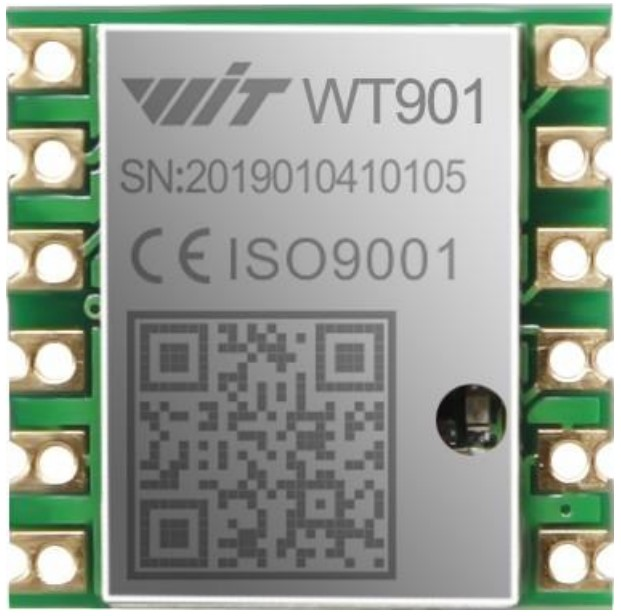
\includegraphics[width=0.8\textwidth]{figures/elec/wt901b.jpg}
        \caption{wt901b}
        \label{fig:WT901B}
    \end{figure}
\end{minipage}
\hfill
\begin{minipage}{0.75\textwidth}
    Ce module regroupe, un accéléromètre trois axes (\(\pm\SI{16}{\g}\)), un gyromètre trois axes
    (\(\pm\SI{2000}{\degree\per\second}\)), un magnétomètre trois axes (\(\pm\SI{4900}{\micro\tesla}\)) ainsi qu'un baromètre. Sa
    particularité, et la raison principale de son choix, est qu'il n'expose pas uniquement des mesures brutes : un microcontrôleur
    interne exécute un algorithme de fusion de type filtre de Kalman et restitue directement l'attitude du module, sous forme
    d'angles d'Euler et de quaternion. Le constructeur annonce une précision angulaire de \SI{0.05}{\degree} sur les axes X et Y,
    et de \SI{1}{\degree} sur l'axe Z après calibration magnétique.\\
\end{minipage}

\vspace{0.2cm}

La communication avec le séquenceur s'effectue par liaison \acrshort{UART} sur un port dédié de la carte. Le module émet
spontanément ses trames, à une cadence configurable de \SI{0.2}{\hertz} à \SI{200}{\hertz}.

\vfill

[METTRE PHOTO SEQUENCEUR]

\vfill

\newpage
